\documentclass{article}

\usepackage{caption,color,fancyvrb,subfig}
\usepackage{code,algorithmic,algorithm}
\usepackage{graphicx,epsfig}
\usepackage{amsmath,amsthm,amsfonts}
\usepackage{amssymb}
\usepackage{setspace}
\usepackage{bibentry}
\usepackage{ulem}

\nobibliography{prelim}

\textwidth = 6.5 in
\textheight = 9 in
\oddsidemargin = 0.0 in
\evensidemargin = 0.0 in
\topmargin = 0.0 in
\headheight = 0.0 in
\headsep = 0.0 in
\parskip = 0.12in
\parindent = 0.0in


\def\inv{^{-1}}

\newcommand{\reminder}[1]{{\bf
    [\marginpar[\hbox{{\Huge
    $\bullet$}\raisebox{0ex}{\Huge $\longrightarrow$}}]%
{\hbox{\raisebox{0ex}{\Huge $\longleftarrow$}{\Huge $\bullet$}}}#1]}}
\newcommand{\pjk}[1]{{\bf
    [\marginpar[\hbox{{\textcolor{blue}{pjk}}\raisebox{0ex}{\Huge $\rightarrow$}}]%
{\hbox{\raisebox{0ex}{\Huge $\leftarrow$}{\textcolor{blue}{pjk}}}}\textcolor{blue}{#1}]}}
\renewcommand{\pjk}[1]{\textcolor{blue}{[#1]}}
\newcommand{\pete}[1]{\textcolor{red}{#1}}
\newcommand{\change}[2]{\sout{#1} \textcolor{red}{#2}}


\begin{document}

\begin{titlepage}
\begin{center}

\textsc{\huge \bfseries \sc{Responsive Consistency in Heterogenous,}}\\
\textsc{\huge \bfseries \sc{Wide Area Distributed Storage Systems}}\\[1.0cm]

\emph{A prospectus submitted in partial fulfillment of the degree of Doctor of
Philosophy}\\[5.5cm]

\textsc{\large DRAFT}\\
\emph{October 19, 2016}\\[2.0cm]

\emph{Preliminary Oral Examination for}\\
\textsc{\large Benjamin Bengfort}\\[2.0cm] % [4.0cm]
\emph{Advisor:} \\
\textsc{Dr. Peter J. Keleher}\\[.5cm]
\emph{Committee Members:}\\
\textsc{Dr. Bobby Bhattacharjee}\\
\textsc{Dr. Dave Levin}\\
\textsc{Dr. Neil Spring}\\[4.0cm]

{\bfseries Department of Computer Science}\\
{\bfseries University of Maryland, College Park, MD 20742}\\
{\bfseries December 9, 2016}
\vfill

\end{center}
\end{titlepage}

\newpage
\thispagestyle{empty}
\mbox{}


\newpage
\setcounter{page}{1}
\onehalfspacing
\begin{abstract}

\pjk{Not tied to rest of para.}Data-oriented consistency models are not a discrete set of various levels, weak, eventual, causal, strong etc. but rather a continuum that can be adapted in response to environmental conditions. Recent studies of consistency have focused on data center environments which are low latency, high bandwidth, and generally stable; and as a result data distribution involves a relatively \pjk{Seems to be a broad statement that is not true when individual jobs might use thousands.}small network of devices. I propose to study consistency in a user-oriented context composed of heterogenous devices (mobile phones, desktops, laptops, cloud storage) that can be mobile, creating a network topology of highly variable latency with routine failure\pjk{s} and whose networks are larger than typically studied - dozens to hundreds of replica servers.\pjk{I think you are talking consensus protocols, not replication protocols, but noone else will know this.}

Our primary context will be a file system that exposes close-to-open consistency and tracks writes to individual objects as a sequence of versions structured as a tree. We consider strong consistency to be a linear sequence of ordered version numbers and inconsistencies to be the presence of forks, misordering, duplicates, or omissions in the version sequence (in order of severity). Additionally we consider the availability of such a system and recognize that enforcement of a linear ordering leads to high latency making the system unusable.

\pete{I/we contend that achieving progress in consensus protocols is highly dependent on the network environment, and that existing protocols can fail to achieve progress in many environments outside the data center.}
\sout{I propose that consistency is primarily related to the network environment as much as it is related to the implemented protocol and as a result, that it can respond the the environment.} By creating a system that has a strong central core that maintains a globally consistent view and allowing other replica servers to be flexible I hypothesize that the system will be more consistent than its homogeneous counterparts reducing the number of forks, misordering, duplicates, and omissions as well increasing the throughput and availability of accesses in the system. I propose two primary mechanisms to make this happen:
\pjk{You are conflating a couple things here, consistency of a log, vs consistency of a file system. The latter is a complex topic that has yet to be introduced. I do think the FS is primary, though it should be clear that a) not limited to FS, and b) the problem is caching (single sentence).}
\begin{enumerate}
    \item \textbf{Federated Consistency}: allow multiple consistency models for different replica servers, integrating over different aspects: temporal, spatial, and synchronization to create a flexible topology of devices with different characteristics and nodes.
    \item \textbf{Hierarchical Consensus}: distribute consensus decisions of sequential ordering in order to make stronger consistency more available.
\end{enumerate}

The experimentation on and development of multi-modal replication protocols via a holistic view will have a large impact in both the data center context as well as in personal distributed file systems.

\end{abstract}
\setstretch{.5}

\newpage
\setcounter{tocdepth}{2}
\tableofcontents

\newpage
\listoffigures

\newpage
\onehalfspacing

\section{Introduction}

The rise of virtualized, on-demand computing resources and cloud computing has dramatically shifted the focus of research on consistency in distributed storage systems away from networked file systems toward geographically distributed database management systems, particularly key-value storage. These types of data systems benefit from low-latency, high-bandwidth connections where failure is common due to the magnitude of resources rather than inherent instability. Because most distribution protocols that provide consistency guarantees are dependent on timing parameters related to the latency of messages, it can be shown that consistency is more dependent on network environment than specific protocols \pjk{Again, not true, unless limiting ourselves to EC, which you don't say.}. As a result, ``eventually consistent'' \cite{vogels_eventually_2009} systems are said to be consistent enough for most workloads given some probabilistic bounding of staleness \cite{bailis_quantifying_2014,bermbach_eventual_2011,bailis_probabilistically_2012}. This has led consistency research towards investigating stronger forms of eventual consistency, primarily building upon Dynamo \cite{decandia_dynamo:_2007} and Cassandra \cite{lakshman_cassandra:_2010} as reference implementations. Alternatively, research into ensuring strong, sequential consistency \pete{or linearizability} in this environment has led to systems like Spanner \cite{corbett_spanner:_2013} which uses atomic and GPS clocks to ensure ``TrueTime'' for sequential ordering or a small number of master nodes that implement consensus algorithms \cite{lamport_paxos_2001,ongaro_search_2014} for locking or ordering \cite{kraska_mdcc:_2013}.

Unfortunately the focus on data center consistency has led to a centralized approach to data storage, forcing a modality where devices must connect to the cloud for file replication even when files exist in the local area \cite{drago_inside_2012}. Although this allows systems to ignore annoyances such as local network configuration and decentralized protocols it does present unnecessary overhead in terms of cost and latency. More pernicious, perhaps, is that users must now buy-in and store their data with a single provider that could go out of business or be hacked, which has lead to research in replicating local data with multiple untrusted cloud stores \cite{zhang_viewbox:_2014,feldman_sporc:_2010}. There are more devices than ever before connecting to storage applications, partially because users have multiple, heterogenous devices from wearables to workstations and partially because of the advent of the Internet of Things \cite{miorandi_internet_2012}. Cloud storage tends to be application specific, but with more devices and more users, generalized distributed storage is required for collaboration and sharing that is not siloed and can be easily accessed by a variety of new platforms.

We propose to explore consistency mechanisms in \textit{user-centric dynamic clouds}: a multi-user tapestry of mobile, heterogenous devices connected via variable-latency and partition-prone networks that change over time. \pete{These clouds are neato, but} We believe that the unique challenges of this environment require specialized consistency models in order to be effective. Because of the user-centric nature of this research and the requirement for generalization\pjk{huh?}, we further propose the study of a file system as the primary data storage application in such networks, particularly as collaboration and sharing make sense for a file system application. File systems must be highly available such that a user does not notice any delay due to coordination but must also have strong consistency such that any conflicts are presented to the user as soon as possible. To that end, our consistency model must be \textit{responsive} \pjk{Seems very important, but buried.} to the network environment providing flexibility when the network is unavailable or laggy and providing strong consistency guarantees when stable connections exist.

Our approach focuses on two primary techniques to provide responsiveness: the \textit{federation} of weak but available consistency mechanisms with sequential consistency by consensus and the \pete{use of} \textit{hierarchical} \pete{consensus} \sout{coordination of quorums so as} to scale \pete{consensus groups} \sout{quorums} beyond a handful of devices \pjk{Is it term you want to use consensus or quorums? I'd think the former}, and to minimize conflict by creating localities of interest with global guarantees\pjk{Important, and comes out of nowhere.}. We hypothesize that the integration of multi-modal consistency \pjk{with....} will lead to higher availability than strong consistency models but provide stronger guarantees than eventually consistent systems. We will quantitatively demonstrate the efficacy of such a system via simulation and by implementing a file system, FlowFS, and testing it under real-life workloads.  By comparing FlowFS to homogenous systems with similar sizes and topologies and measuring the number of inconsistencies and amount of latency in both simulation and a real world implementation we will show that responsive, flexible consistency protocols are more available and provide stronger guarantees than their homogenous counterparts in user-centric dynamic personal cloud topologies.

\section{Background and Related Work}

Our work is motivated by open questions \pjk{??} related to data-centric consistency models, previously thought of as discrete levels but now viewed as a continuum along the dimensions of ordering and staleness \cite{bermbach_consistency_2013}. We will start by defining our consistency model and our primary metric: \textit{forks}. By presenting various consistency levels on this continuum, we will provide background to our first responsive approach: Federated Consistency: a system that implements multiple consistency models either on demand or in response to observations about the state of the network.

Federated Consistency requires a strong central core in order to provide stronger global guarantees, similar to the architecture presented in Oceanstore \cite{kubiatowicz_oceanstore:_2000}. The central core requires a consensus algorithm to ensure that they maintain a sequentially ordered state, one that can scale to larger systems than those typically studied. In order to provide background on Hierarchical Consensus, we will present several consensus algorithms and discuss their performance improvements and benefits. Finally, we will review topics in replication, critical to our work and present related systems already implemented.

\subsection{Consistency}

% Should I review the client-centric consistency models

\pjk{really, really need to distinguish between log and FS consistency. Someone just reading this for the first time might not understand why consensus doesn't give you perfection. You \emph{must} address this briefly up front, and then in more detail later.} 
Our consistency model is a \textit{data-centric} model (as opposed to a \textit{client-centric} model) which can be described by two primary facets: ordering and staleness \cite{bermbach_consistency_2013}. We generalize consistency as follows: every replica server maintains a single, ordered log of accesses (reads and writes) to multiple named objects. Each log entry refers to a \textit{version} of that object, specified as a monotonically increasing, conflict-free version number and a parent version. A read of an object name searches the log in reverse order and returns the first version from the end referring to that name. A write to an object creates a new version from an earlier parent version. As accesses interact with object versions and append to the log, we can characterize the consistency facets as follows:

\begin{enumerate}
    \item \textit{Ordering} refers to how closely individual logs adhere to the abstract global ordering. A \textit{strict ordering} requires every single log to be exactly the same \pjk{or a prefix?} whereas weaker ordering allows some divergence in the order writes are stored in the log.
    \item \textit{Staleness} refers to how far behind the latest global version a local log is and can be either expressed by the visibility latency of replicating a version to all replicas or simply by how many versions the latest is behind by.
\end{enumerate}

\begin{figure}
    \centering
        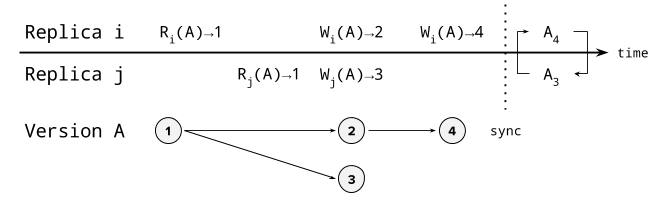
\includegraphics[width=.9\textwidth]{figures/forks}
        \caption{Forks branch sequentially ordered version numbers}
        \label{fig:forks}
\end{figure}

Most data-centric consistency models \pjk{cite} do not consider staleness but instead refer to the strictness of ordering guarantees and the method by which updates are applied to the state of the replica. Indeed, ordering strictness can lead to to increased staleness because writes cannot be accepted until they have fulfilled their dependencies first, creating further delay. However, log ordering is difficult to quantify, therefore our consistency model considers instead the primary symptom of stale reads and writes: \textit{forks}.

\begin{description}
    \item[\textbf{Fork}] A fork occurs when two replicas concurrently write a new version to the same parent object as shown in Figure \ref{fig:forks}. Forks introduce inconsistency because there are now two potential orderings of updates to the log, but forks are primarily the symptom of staleness; e.g. the second writer wrote to a stale version of the object.
\end{description}

There are two primary causes of forks: concurrent accesses by multiple replicas (a true conflict between multiple writers) and stale reads. The former is distinguished from the latter only if the possibility of synchronization (a process to bring replica logs to the same state) could have occurred. From the point of view of the system, they are identical causes. Forks can branch to arbitrary lengths as replicas continue to write to their latest local copies, however when synchronization occurs a decision as to which ordering of writes is correct must occur. With this context and consistency model in mind, we can now identify several consistency models in order of increasing ordering strictness and define how each model's correctness criteria responds in the face of forks.

\subsubsection{Discrete Consistency Levels}

\pjk{You are talking about consistency wrt to logs, not in general, so say that.}
\textit{Weak consistency (WC)} is is the least strict consistency model.
A weakly consistent system makes no guarantees whatsoever about the relationship of local \sout{vs.} \pjk{never use abbreviations} remote writes and whether or not any given update will become visible \cite{vogels_eventually_2009}. Weak consistency is often described as ``replicas might get lucky and become consistent'' and in fact a weakly consistent implementation may not have a synchronization protocol whatsoever \cite{bermbach_consistency_2013}. For this reason, we do not consider weak consistency in general except to identify it as a baseline.

\textit{Eventual consistency (EC)} is primarily concerned with the final state of all logs in the system given some period of quiescence that allows the system to converge. In this case, all replicas, no matter their log ordering, should have identical final versions for all objects \sout{in the namespace}\pjk{not introduced yet}. This suggests that eventual consistency requires some \textit{anti-entropy} mechanism to propagate writes and a policy to handle convergence \cite{terry_managing_1995}. Eventual consistency is very popular for NoSQL databases and hosted distributed storage services \cite{decandia_dynamo:_2007,lakshman_cassandra:_2010} because it \change{favors}{allows} an optimistic approach to consistency: \change{in most systems conflicts are rare}{conflicts are rare in most systems} \sout{and } if something does go wrong, conflict resolution is passed to the application layer. In practice, most applications can handle some inconsistency and moreover the small inconsistency windows due to low latencies in cloud data centers make such conflicts rare and short-lived enough to be worth the risk \cite{bailis_quantifying_2014}.

Eventual consistency implemented by a \textit{last writer wins} policy simply accepts all writes so long as they are more recent than the latest local versions. Eventual reads and writes are always performed on local caches and are therefore highly available since they return a response to accesses immediately. Eventual consistency does allow forks to occur and moreover allows individual replica logs to have wholly different orderings so long as the last version for each object is in the same given no accesses have occurred for a long enough period of time. As a result, the latest version of an object may alternate between writes to competing forks (a fairly weak semantic) and in this case, it is up to the application to detect the inconsistency. However, EC logs do have one important property - for each object, every write in the log is ordered in a monotonically increasing fashion.

\textit{Causal Consistency (CC)} ensures that all writes which have causal relationships have those dependencies satisfied (inserted into the log) before the write can become visible \cite{ahamad_causal_1990}. Therefore, even though a write might have been propagated to another replica server it cannot be read until all of its dependencies have also been propagated. Causal consistency can increase staleness particularly when implicit or potential causality creates large dependency graphs that must be resolved before writes can be applied \cite{lloyd_dont_2011}. This can be managed by allowing the application to explicitly specify the dependencies for each write \cite{bailis_potential_2012}. Causal consistency is often referred to as the ``strongest form of consistency for highly available systems'', however CC does not require replica convergence \cite{guerraoui_consistency_2002} though with a few modifications including a convergence mechanism, it can easily be bolted on to an eventual system \cite{bailis_bolt-causal_2013}.

Eventual and causal consistency are both weak forms of consistency that are designed for high availability; that is they can respond to requests immediately from a local cache without coordination. Conflict detection and resolution are therefore critical processes asynchronous with the accesses that cause the conflict. These types of consistency are well suited for network environments that are partitioned or such that effective coordination is not available at the time of the access; e.g. for a user working on an airplane with no connectivity. The following strong consistency models, on the other hand, require coordination at the time of the access, detecting and eliminating conflict synchronously.

\textit{Sequential consistency (SC)} is a strong consistency model that requires that all replicas have the exact same ordering of their logs, such that all writes by all clients are appended in the same exact order \cite{attiya_sequential_1994}. Sequential consistency is not strict in that it does not make guarantees about staleness (or the ordering of reads) but does require that all writes become visible in the same order \cite{bermbach_consistency_2013}. Sequentially consistency is typically implemented with consensus algorithms such as Paxos \cite{lamport_fast_2006} or Raft \cite{ongaro_search_2014} that coordinate logs by defining a transitive, global ordering for all conflicts. Alternatively, sequential consistency and can be implemented with warranties -- time based assertions about a group of objects that must be met on all replicas before the assertions expired \cite{liu_warranties_2014}.

\textit{Linearizability (LIN)} is the strongest form of consistency; not only must all write operations occur in sequence, but all operations including reads must be ordered chronologically \cite{herlihy_linearizability:_1990}. A consensus algorithm alone cannot implement linearizability and instead some distributed locking mechanism is required. For example a consensus algorithm can be adapted to instead of making decisions about the total ordering of conflicting writes, granting or releasing locks from requestors, however this opens up the potential for deadlock and extremely poor performance, defeating the purposes of replication in the first place! Data center environments that don't have to deal with issues of clock skew by using super precise atomic and GPS clocks can use precise time measurements to enable a distributed two phase commit protocol \cite{corbett_spanner:_2013}, however every replica is required to have such a time piece, which is not practical for heterogenous topologies.

\subsubsection{Consistency Rationing and Hybridization}

Federated Consistency attempts to integrate multiple consistency levels as described in the previous section into a hybrid consistency model such that there is a separation between the local availability and consistency trade-off and global consistency guarantees. For example, the hybridization of an eventual consistency cloud of devices with a strong sequential core allows eventual nodes to make progress, while minimizing the effect of convergence delay on consistency. In this section, we will review work related to this style hybridization.

One of the earliest attempts to hybridize weak and strong consistency was a model for parallel programming on shared memory systems by Agrawal et al \cite{agrawal_mixed_1994}. This model allowed programmers to relax strong consistency in certain contexts with causal memory or pipelined random access in order to improve parallel performance of applications. Per-operation consistency was extended to distributed storage by the RedBlue consistency model of Li et al \cite{li_making_2012}. Here, replication operations are broken down into small, commutative suboperations that are classified as red (must be executed in the same order on all replicas) or blue (execution order can vary from site to site), so long as the dependencies of each suboperation are maintained. The consistency model is therefore global, specified by the red/blue ordering and can be adapted by redefining the ratio of red to blue operations, e.g. all blue operations is an eventually consistent system and all red is sequential.

The next level above per-operation consistency hybridization is called \textit{consistency rationing} wherein individual objects or groups of objects have different consistency levels applied to them to create a global quality of service guarantee. Kraska et al. \cite{kraska_consistency_2009} initially proposed consistency rationing be on a per-transaction basis by classifying objects in three tiers: eventual, adaptable, and linearizable. Objects in the first and last groups were automatically assigned transaction semantics that maintained that level of consistency; however objects assigned the adaptable categorization had their consistency policies switched at runtime based on a cost function that either minimized time or write costs depending on user preference. This allowed consistency in the adaptable tier to be flexible and responsive to usage.

Chihoub et al. extended the idea of consistency rationing and proposed limiting the number of stale reads or the automatic minimization of some consistency cost metric by using reporting and consistency levels already established in existing databases \cite{chihoub_harmony:_2012,chihoub_consistency_2013}. Here multiple consistency levels are being utilized, but only one consistency model is employed at any given time for all objects, relaxing or strengthening depending on observed costs. By utilizing all possible consistency semantics in the database, this model allows a greater spectrum of consistency guarantees that adapt at runtime.

Al-Ekram and Holt \cite{al-ekram_multi-consistency_2010} propose a middleware based scheme to allow multiple consistency models in a single distributed storage system. They identify a similar range of consistency models, but use a middleware layer to forward client requests to an available replica that maintains consistency at the lowest required criteria by the client. However, although their work can be extended to deploying several consistency models in one system, they still expect a homogenous consistency model that can be swapped out on demand as client requirements change. Additionally their view of the ordering of updates of a system is from one versioned state to another and they apply their consistency reasoning to the divergence of a local replica's state version and the global version. Similar to SUNDR, proposed by Li et al. \cite{li_secure_2004}, an inconsistency is a fork in the global ordering of reads and writes (a ``history fork''). Our consistency model instead considers object forks, a more granular level that allows concurrent access to different objects without conflict while still ensuring that no history forks can happen.

Hybridization and adaptation build upon previous work that strictly categorizes different consistency schemes. An alternative approach is to view consistency along a continuous scale with a variety of axes that can be tuned precisely. Yu and Vahdat \cite{yu_design_2002} propose the \textit{conit}, a consistency unit described as a three dimensional vector that describes tolerable deviations from linearizability along staleness, order error, and numeric ordering. Similarly, Afek et al. \cite{afek_quasi-linearizability:_2010} present quasi-linearizable histories which specify a bound on the relative movement of ordered items in a log which make it legally sequential.

\subsection{Consensus}

Consensus algorithms are generalized as replicated state machines where a quorum of replicas must coordinate to decide on the application of a command that will change the local state of the replica \cite{schneider_implementing_1990}. By keeping a log of all applied commands, consensus is fault-tolerant because an offline node that rejoins the quorum can replay the commands to return to the same state as the other replicas; consistency in this context is that all replicas share the same state. Moreover, so long as a majority of nodes are online, the quorum can be said to be available, in that it will respond to requests that access the state. Because accesses can be seen as commands modifying the visible state of the object namespace, and because the command log is identical to the consistency logs described in the last section, we can say that consensus algorithms can be used to provide strong consistency at the cost of multiple coordination messages per access.

Most consensus algorithms in the literature are variations of the Paxos algorithm, and more specifically the Fast Paxos implementation \cite{lamport_fast_2006}. Paxos proposes three phases in the application of a command to the state machine: \textit{prepare}, \textit{propose}, and \textit{accept}. All phases are two stages, the first a vote and the second a broadcast of the results of the vote. In the prepare phase, a replica attempts to establish the master replica for a specific command by broadcasting a ballot number and getting majority agreement that the ballot (the entry at the log at that position) is owned by the master. The second phase broadcasts the value and receives a majority vote if that state can be successfully applied. The third phase accepts (commits) the result to the state machine. The primary variation, Fast Paxos, bundles multiple requests by reserving ballot numbers ahead of time to eliminate the \textit{prepare} phase (which is why most descriptions of Paxos generally identify only two phases). One way we can think of this is as the election of a primary leader in the quorum.

Because of the multiple round-trips necessary to achieve consensus, many variations of Paxos have been proposed to improve performance. For example S-Paxos \cite{biely_s-paxos:_2012} attempts to distribute the workload of the leader, Multi-Paxos \cite{camargos_multicoordinated_2007} allows multiple leaders per round, Flexible Paxos \cite{2016arXiv160806696H} allows for multiple quorum intersections, and Egalitarian Paxos \cite{moraru_egalitarian_2012,moraru_there_2013} allow fast and slow track voting. These variations tend to be optimistic in that conflict occurs rarely and that it can be detected by the consensus algorithm, allowing for repair if necessary.

\subsubsection{Raft}

Paxos has been shown to be very difficult to correctly implement and verify \cite{chandra_paxos_2007} and although attempts have been made to highlight the practicality of a subset of the Paxos guarantees \cite{mazieres_paxos_2007} it has been shown that Paxos is not easily understandable. To that end, we have used the Raft consensus protocol \cite{ongaro_search_2014, howard_raft_2015} as our primary consensus implementation in our preliminary investigations. The protocol is described briefly as follows.

Every Raft node can be in one of three states: \textit{follower}, \textit{candidate}, and \textit{leader} and are initialized in the follower state. The system has two primary timing parameters: the election timeout and the heartbeat interval. When in follower and candidate mode, a timeout is randomly selected from the election timeout range, and if the timeout occurs the node will become a candidate and start an election to become leader. If a majority of nodes vote yes to that candidate then the node switches to the leader state and begins sending \texttt{AppendEntries} messages at the rate of one at least every heartbeat interval. If a follower or a candidate receives a valid \texttt{AppendEntries} message, it resets its election timeout by selecting a new random timeout from the election timeout range. The relationship between the heartbeat interval and the election timeout must be such that at least two heartbeats can arrive before the node switches to candidacy. The random selection of a timeout prevents thrashing if all nodes are started at the same time.

Once elected leader, all accesses are forwarded to that node. Leaders maintain a term identification, a monotonically increasing global number. If a message comes in with a remote term higher than the local, then that node must switch to being a follower and update their local term. Accesses and their terms are sent to all followers in \texttt{AppendEntries} messages. Followers compare their terms to the access term, and if a majority of followers accept the access, then the leader sends a commit message in the following \texttt{AppendEntries} RPC message.

% \subsubsection{Consensus Trees}
% NOTE: Wanted to put in related works, similar to consistency discussion.

\subsection{Replication}

\pjk{Explicitly distinguish between metadata and data. Also mention immutable data chunks as a way to show that consistency in data is unimportant.} Consistency and consensus are generally separate issues from the actual replication of data in a distributed storage system. For example, causal consistency does not have a convergence mechanism described explicitly. There are two primary methods we have explored for replicating data in a distributed file system: gossip protocols and broadcast protocols. Gossip protocols are generally used in anti-entropy to disseminate information across the network in an epidemic fashion. Broadcast replication can quickly overwhelm a system if all nodes are broadcasting, but is used well in centralized systems such as the Raft protocol.

Gossip protocols (often called rumor spreading) are a form of epidemic information spreading that do not require central coordination \cite{kempe_gossip-based_2003, karp_randomized_2000}. On a routine interval, specified by the \texttt{anti-entropy delay} timing parameter, a replica will randomly select one of the other replicas in the system and exchange information. Because all nodes are randomly selecting another node at every interval, information travels quickly through the network in an exponential fashion and provide high fault-tolerance and even automatic stabilization. Generally speaking there are two types of gossip: \textit{push} and \textit{pull}. Push methods simply forward all locally updated information to the remote node on the anti-entropy interval. Pull methods require two phases: a request for information after a certain period and the response from the remote node.

Several replication protocols have directly influenced or inspired our work. Bayou \cite{terry_managing_1995,terry_session_1994} is an eventually consistent system that implements anti-entropy as its replication mechanism and conflict resolution by some primary or trusted centralized server. SUNDR \cite{li_secure_2004} is a secure file system that integrates local and cloud storage and detects inconsistencies by identifying forks, our primary inconsistency metric. The Ori File System \cite{mashtizadeh_replication_2013} replicates file history and allows the merge and grafting of histories similar to Git trees. As a result branches and forks are also a big part of the Ori methodology as are complex data structures for grafting and dealing with conflict. Finally, the Stellar consensus protocol \cite{mazieres_stellar_2015} provides federated byzantine agreement through the use of quorum slices.

\section{Preliminary Work}

\pjk{Federated!} We have begun our investigation into the relationship between network environment and consistency by building a discrete event simulator in Python using SimPy that allows us to easily characterize networks and consistency protocols. The simulator has two primary components: workload generators, which act as users that issue read and write accesses to named objects and device processes, which are connected to each other via a specified topology, respond to accesses, generate replication messages, and respond to messages from other devices. Experiments are conducted by running multiple simulations in parallel with different parameters, topological configurations, and accesses. Analysis is conducted on the results of a single simulation or on multiple simulations.

\begin{figure*}
    \centering
    \minipage{0.48\textwidth}
      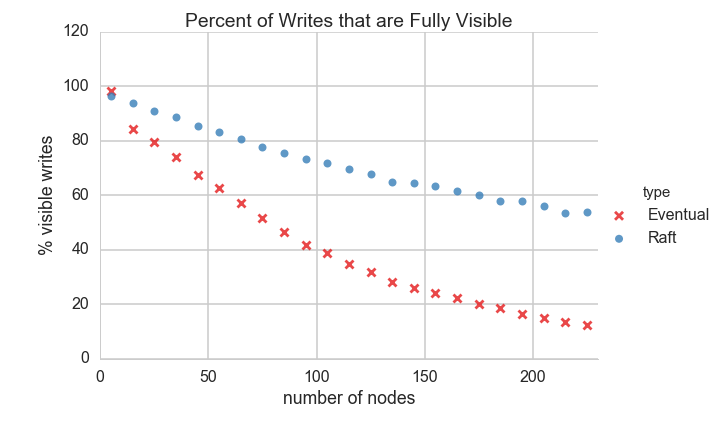
\includegraphics[width=\linewidth]{figures/scaling/visible_writes}
      \caption{Percent of fully visible writes in homogenous eventual and sequential consistency systems.}
      \label{fig:scaling_visible_writes}
    \endminipage\hfill
    \minipage{0.48\textwidth}
      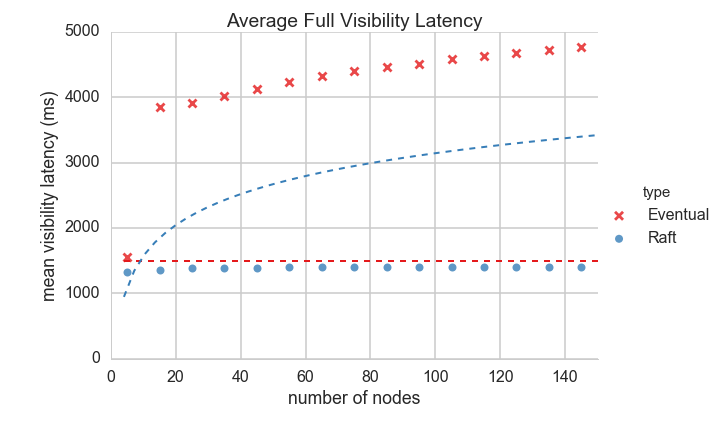
\includegraphics[width=\linewidth]{figures/scaling/visibility_latency}
      \caption{Latency of full visibility in homogenous eventual and sequential consistency systems.}
      \label{fig:scaling_visibility_latency}
    \endminipage
\end{figure*}
\pjk{All text in figures, including data points, need to be larger.}
Because most research on gossip protocols and quorums specifies small quorums of a size that provide a minimum fault tolerance, our first question related to the effect of consistency protocols with increasing numbers of nodes. We created two homogenous distributed systems: an eventual consistency system implemented with anti-entropy via bilateral gossip and a latest-writer wins policy and sequential consistency by consensus implemented using the Raft consensus algorithm. Each simulation varied the number of nodes in one of five locations, e.g. 5 nodes had one node per location, 25 with 5 nodes per location, up to 100 with 20 nodes per location. Local area latencies were normally distributed with the mean latency, $\lambda_{\mu}=30$ms and the standard deviation of latency, $\lambda_{\sigma}=5$ms whereas wide area latencies were higher and more variable, $\lambda_{\mu}=300$ms and $\lambda_{\sigma}=50$ms.

The timing parameters for both Eventual and Raft are based on \sout{the} network latency. We first computed a conservative timing parameter, $T=10\lambda_{\mu}$ based on the wide area latency mean. The anti-entropy interval for Eventual consistency is given as $\frac {T} {4} = 750$ms. For Raft, the heartbeat interval is $\frac {T} {2} = 1500$ms and the election timeout is a uniform random selection in the range $U(T, 2T) = U(3000, 6000)$. These conservative timing parameters ensure that it is rare that messages arrive out of order.

As the number of nodes increases, both Raft and Eventual systems start to degrade in terms of the percent of writes that are fully visible as shown in Figure \ref{fig:scaling_visible_writes}. For Eventual, this is because the time to visibility is related to the number of pairwise anti-entropy sessions required to propagate a write to all nodes as shown in Figure \ref{fig:scaling_visibility_latency}, where the blue line represents perfect convergence (not likely given uniform random neighbor selection). Raft on the other hand has a broadcast mechanism related to its heartbeat interval but writes do not become fully visible because they are rejected by the leader as inconsistent.

\begin{figure*}
    \centering
    \minipage{0.48\textwidth}
      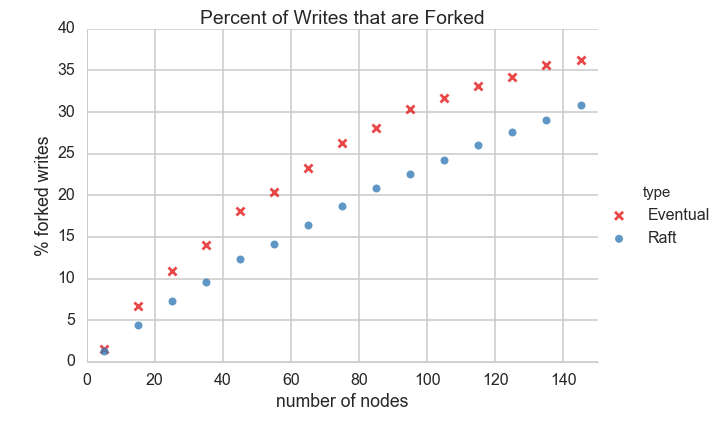
\includegraphics[width=\linewidth]{figures/scaling/forked_writes}
      \caption{Increasing forks in homogenous systems as topology size increases.}
      \label{fig:scaling_forked_writes}
    \endminipage\hfill
    \minipage{0.48\textwidth}
      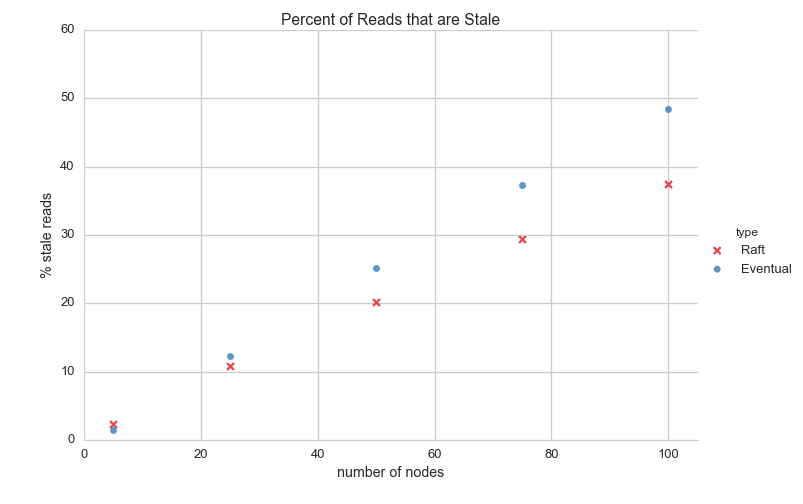
\includegraphics[width=\linewidth]{figures/scaling/stale_reads}
      \caption{Increasing stale reads in homogenous systems as topology size increases.}
      \label{fig:scaling_stale_reads}
    \endminipage
\end{figure*}

Read and write accesses were conducted on each device on 15 objects such that the probability of conflict, $P_c=0.3$ meaning that 30\% of the objects accessed on each device would also be accessed on another device. Accesses were issued at intervals normally distributed with the access interval mean, $A_{\mu}=3000$ms and the access interval standard deviation, $A_{\sigma}=380$ms such that accesses were roughly related to the timing parameter. As the number of nodes increases, the number of conflicts also increase, but not the likelihood of a conflict. Our system measures inconsistencies as \textit{forks} and \textit{stale reads}. As shown in Figure \ref{fig:scaling_forked_writes}, the number of conflicts in Raft is lower than in eventual as are the number of stale reads as shown in \ref{fig:scaling_stale_reads} but at the cost of a performance decrease, particularly as the number of nodes increases.

We believe that these initial investigations show a critical opportunity: that we can blend the high availability of an eventually consistent system and leverage the best parts of anti-entropy and eventual consistency in network environments where messages cannot get through along with the stability and increased visibility of a strongly consistent core, similar to the central core and flexible outer shell proposed by Gray and Oceanstore \cite{gray_dangers_1996,kubiatowicz_oceanstore:_2000}: we call this \textit{Federated Consistency}. Furthermore, if we can find a way to allocate decision space to a smaller number of nodes, we should be able to scale Raft to greater number of nodes without as steep a curve: we investigate this in \textit{Hierarchical Consensus}. Finally, as suggested by the $T$ timing parameter (though not explicitly covered), the timing measures and performance of consistency protocols are related to the network environment, which is dynamic. Potentially we can improve performance by monitoring the environment and adapting timing parameters to minimize the number of inconsistencies: investigated in \textit{Adaptive Consistency}.

\subsection{Topology}

In order to investigate the effect of variable latency and the network environment on consistency, we have constructed a fully connected topology of replica nodes that are each assigned a geographic region as shown in Figure \ref{fig:topology}. Within each region, replica nodes enjoy stable, low-latency connections with their neighbors. However, across regions the latency is higher and the connections variable, meaning that out of order messages are more common across the wide area than in the local area.

\begin{figure*}
    \centering
    \minipage{0.5\textwidth}
      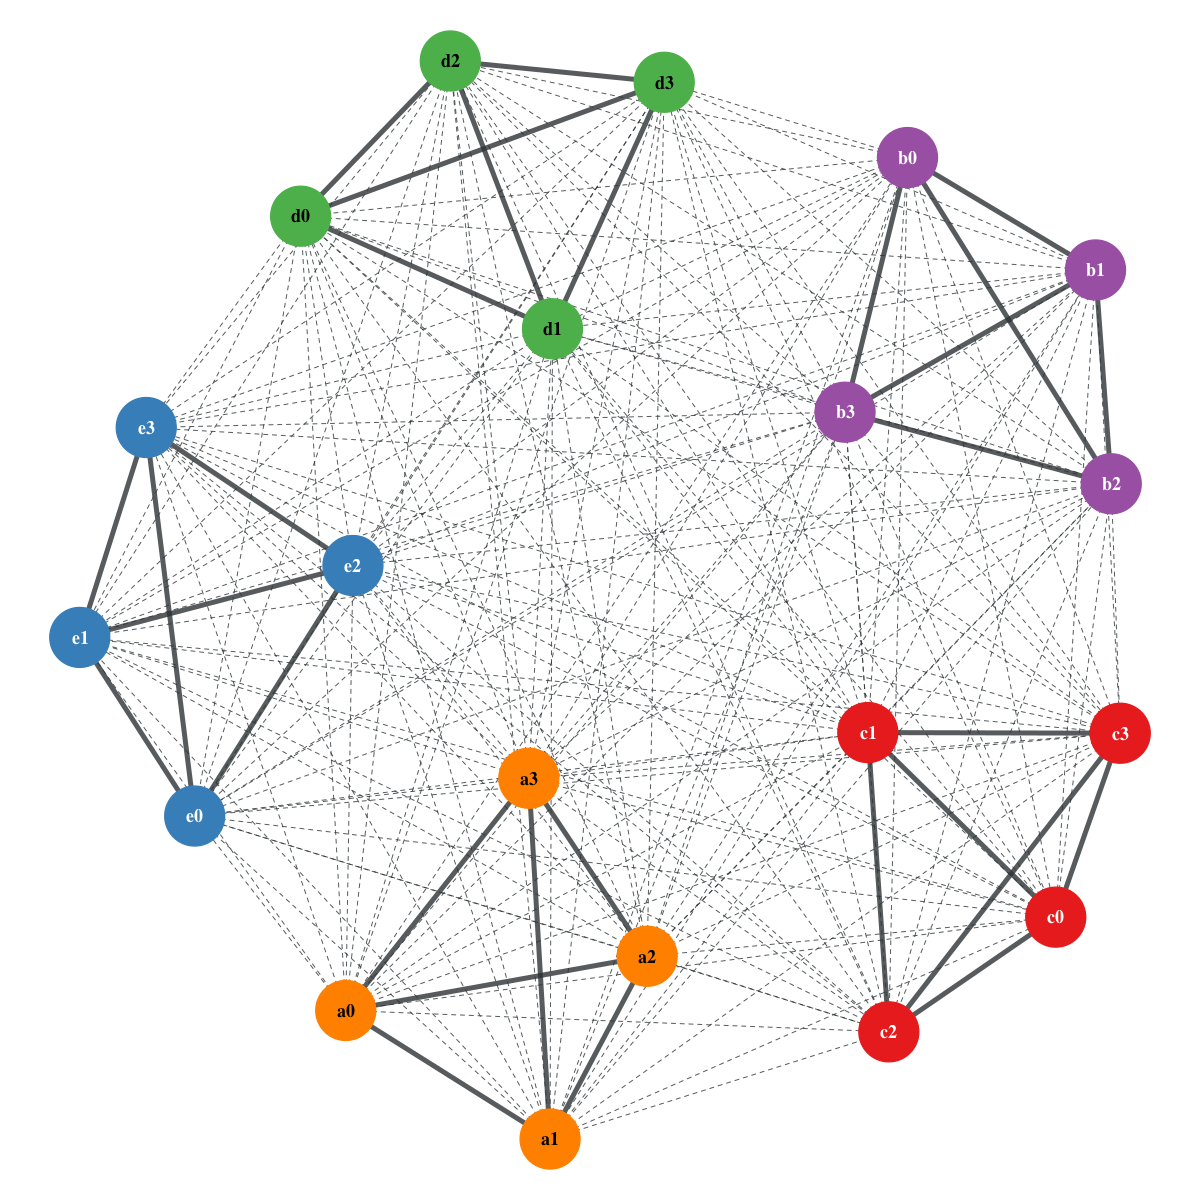
\includegraphics[width=\linewidth]{figures/topology}
      \caption{Proposed Network Topology.}
      \label{fig:topology}
    \endminipage\hfill
    \minipage{0.5\textwidth}
      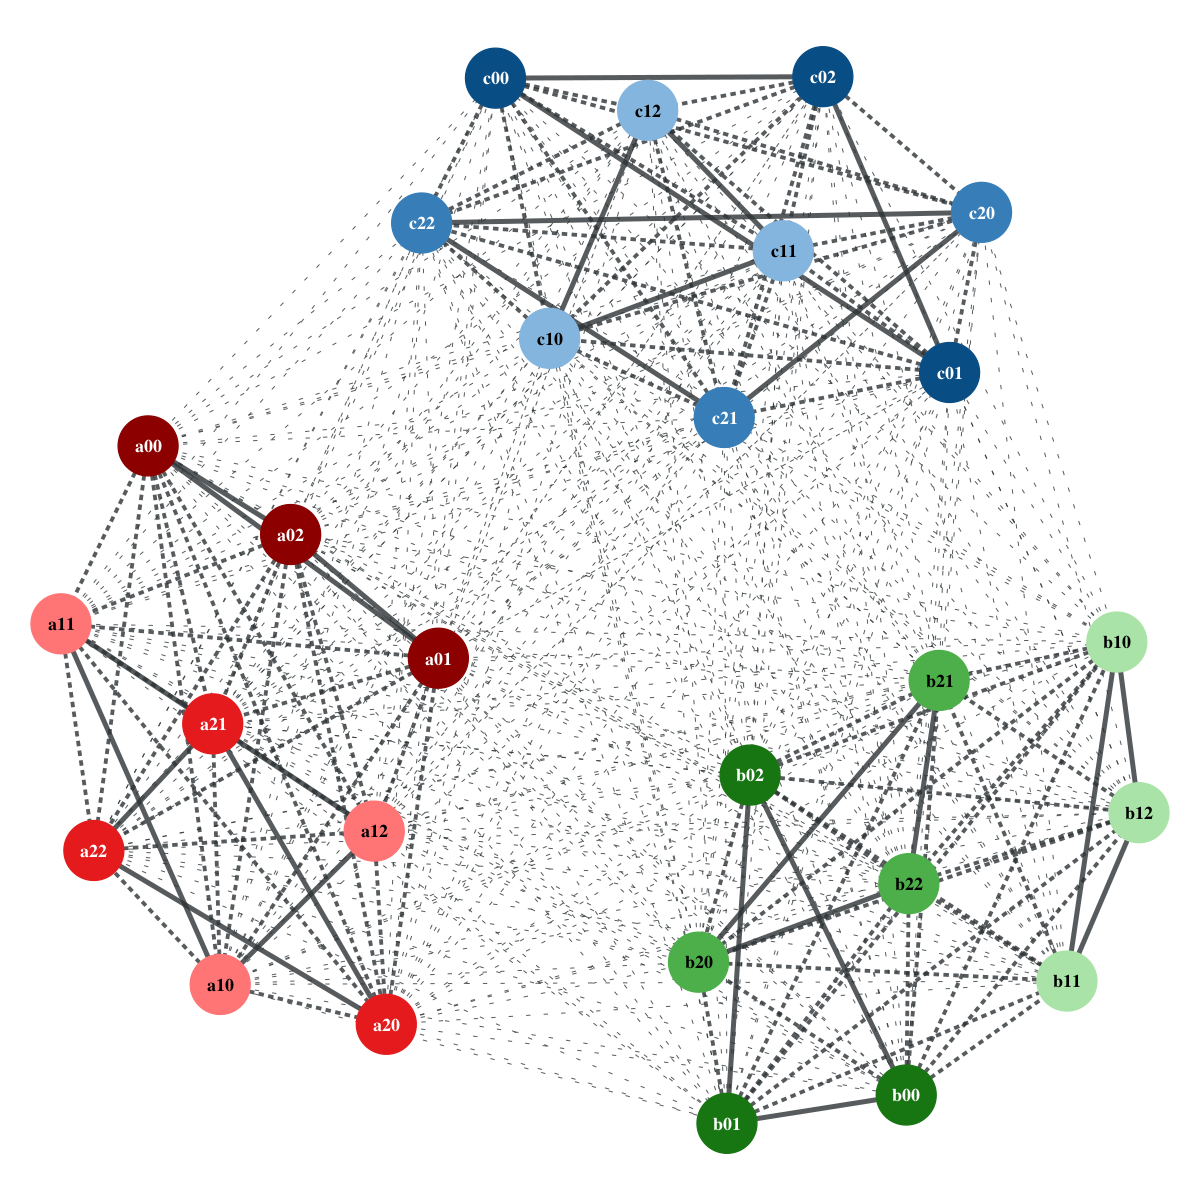
\includegraphics[width=\linewidth]{figures/tiers}
      \caption{Proposed Network Hierarchy.}
      \label{fig:tiers}
    \endminipage
\end{figure*}

In this type of topology there are two types of failure: node failure and network partitions. \textit{Node failure} occurs when a single node is shut off or stops responding to messages. \textit{Network partitions} occur when it is not possible for messages to be sent or received from a single geographic region. In both cases, two conditions must be dealt with by the replication protocol in order to satisfy correctness criteria: first the fact that accesses may continue at a partitioned node which are not being replicated by the system and second that the partitioned nodes are behind the global state and must be brought up to date.

For hierarchical consensus we have introduced a three tier topology consisting of three regions where nodes enjoy two types of network connections as shown in Figure \ref{fig:tiers}. Each region of nine nodes has three inner circles of very high connectivity (e.g. hard lines) while connectivity in the rest of the region is moderate and connectivity across the wide area is variable. This topology will allow us to explore hierarchical models in depth.

\subsection{System Description}

Our file system aggregates individual accesses into \textit{Close-To-Open} (CTO) consistency where read and write accesses are ``whole file'' \cite{muthitacharoen_low-bandwidth_2001}. Furthermore, with respect to local accesses we guarantee that a read returns the last write (given no remote updates, \textit{Read Your Writes Consistency}) and that writes are atomic with respect to each other (\textit{Monotonic Write Consistency}) \cite{bermbach_consistency_2013}.

Each replica's log is composed of a series of write accesses to multiple objects. Each object has a unique name that identifies it to the system and a monotonically increasing version number which can be implemented either as a vector clock \cite{parker_detection_1983} (or a simple Lamport scaler) in the case of a fixed topology or as a vector stamp \cite{almeida_version_2002} in the case of dynamic topologies. Therefore a write access encapsulate the following information: the name of the object being written to, the parent version of the object to which the write is being applied, the versions and object names of any other dependencies, the replica id where the write occurred, and an array of blob ids that compose the file at the conclusion of the write.

A read access to a particular object simply looks up the latest local version of that object. Because dependency information can be embedded into a write, it is not necessary to include read accesses in the log. For example, in order to create a transaction that reads from objects $X$ and $Y$, performs a computation then updates objects $Y$ and then $Z$: the write to $Y$ would include as a dependency the earlier version of $Y$ and the read version of $X$ and the write to $Z$ would include the updated version of $Y$ and the read version of $X$. Other notions of dependencies include implicit session dependencies, e.g. all writes are dependent on any access that occur within a minimum time threshold of each other, or explicit dependencies that are added by the application.

Because our system model accounts for heterogenous devices and each write in the log is simply metadata about the version of a file we consider version replication as a separate issue from object or blob replication. Furthermore, system consistency depends only on the replication of version information since a version defines what is visible on each replica to be read (and writes follow an implicit read). While a version must become visible (replicated to) all devices in order for the system to be consistent, the blobs that make up data may not be stored on all devices with different storage resources. If a read access requires blobs that it doesn't have, it can simply request them from a local neighbor that does, or from the origin replica itself.

\section{Proposed Work}

\pjk{Needs to be stronger.} \sout{In order to} investigate the effects of consistency and scaling in heterogenous, partition prone, variable latency networks we propose to build a distributed file system called FlowFS that implements two primary methodologies: Federated Consistency and Hierarchical Consensus. Federated Consistency allows us to create a flexible, heterogenous distributed system, allowing different replica servers to maintain different consistency levels based on need, but ensuring that global consistency guarantees are met. Hierarchical Consensus extends the Raft consensus protocol \pete{to use consensus partitioning as a means of achieving scale and high availability among replicated logs, without sacrificing sequential consistency} \sout{such that the quorum can scale, providing high availability sequential consistency}. We further propose the stretch goal of the investigation of real time optimization and adaptation in response to changing network environments in mobile contexts. This stretch investigation will explore heuristic methods of optimization and steering configuration changes, as well as explore active, machine learning mechanisms

\subsection{Federated Consistency}

Heterogenous topologies with multiple users mean a variety of requirements for both availability and correctness. For example, consider a user working on a non-critical document on a train with limited cellular connectivity; the requirement here is probably high availability and progress rather than strong replication. On the other hand, during collaborative document editing, users might want to ensure strong sequential consistency and are willing to accept minimal delays such that the document is always in a consistent state. However, it is not possible to maintain a single, global consistency level that meets both of these requirements, leading us to the question: can consistency be adapted or tuned at runtime in such a way as to provide more availability in low connectivity situations or for low conflict objects and strong consistency and correctness in optimal network conditions or for critical or high priority workloads?

% Make sure to show that this is work already underway.
Our preliminary solution is a hybridization of discrete consistency models as discussed earlier, which we have already begun exploring via the simulation as introduced in the preliminary work. The Federated Consistency model allows individual replicas to select their own local consistency policies and engage in replication according to the mechanism specified by the policy. Each replica maintains its own local state which is modified in response to local accesses as well as the receipt of messages from remote replicas. Each replica sends messages to other nodes in order to propagate the latest writes as well as to perform housekeeping. Therefore every replica can be seen as an event handler that responds to local access events as well as remote messages and generates more events (sent messages) in return. Simply put, so long as every federated replica has an event handler for all types of RPC messages, federation only has to be defined at the \textit{consistency boundaries}, that is when replicas of one consistency type send messages to that of another.

Given the consistency models discussed in the previous section, we will omit weak consistency as being too simplistic and linearizability as being too performance restrictive. Instead we will focus on the federation of eventual consistency, implemented with latest-writer wins gossip based anti-entropy, and sequential consistency implemented with the Raft consensus algorithm.

A federated consistency protocol finds a middle ground in the trade-off between performance and consistency, particularly between an eventually consistent system implemented via gossip-based anti-entropy \cite{kempe_gossip-based_2003} and a sequential consistency model implemented by the Raft consensus protocol \cite{ongaro_search_2014}. By exploring these two extremes in the consistency spectrum we have observed in simulation that the overall number of inconsistencies in the system is reduced from the homogenous eventual system and that the access latency is decreased from the homogenous sequential system. Moreover, because the global consistency of the system is topology-dependent, it can be said to have flexible or dynamic consistency. We have found that large systems with variable latency in different geographic regions can perform well by allowing most nodes to operate in an optimistic fashion, but maintain a strong central quorum to reduce the amount of global conflict.

\subsubsection{Gossip and Anti-Entropy}

Eventual consistency \change{provides an option for}{allows} replicas to operate in a highly available fashion at the risk of encountering some conflict (in the form of forks) that must be resolved in the future. \change{Our implementation utilizes} {We take the common approach of using} periodic \textit{anti-entropy} sessions \change{that}{to} converge replicas \sout{towards the same state} (e.g. reducing entropy, the divergence between the states of individual replicas) via \pete{a} gossip protocol \cite{kempe_gossip-based_2003}. \change{On a routine interval, specified by the \texttt{anti-entropy delay} timing parameter, a}{Each} replica \pete{periodically selects a random partner} \sout{will randomly select one of the other replicas in the system} and sends a \texttt{Gossip} message \change{that contains}{containing} the latest version of all objects in the replica's local log. On receipt of the \texttt{Gossip} message, the remote replica will compare the RPC object versions with those in its local log. If the RPC versions are later, it will append the later versions of the object to the log (\textit{last-writer wins}). However if the remote object version is later it will send that version back to the originating node in a \texttt{GossipResponse} message. As a result, our anti-entropy implementation is \textit{bilateral}.

\change{Replicas that implement eventual consistency}{Eventual consistency replicas} \change{read locally and write to their local latest version introducing zero read and write latency}{read and write locally, resulting in essentially read and write latency}. Forks are caused by \sout{staleness due to} the \textit{visibility latency}, i.e., the amount of time \change{it takes}{needed} to propagate a write to the rest of the system. The visibility latency is dependent on the number of nodes in the topology and the anti-entropy interval, but because of the bilateral nature of our gossip protocol, has an exponential distribution rate \pjk{grows exponentially?}. \sout{It is important to note that} the relationship between the anti-entropy delay and the size of the network relative to the mean time between accesses \sout{could} potentially means that eventual consistency would \change{have no}{not cause} forks. Said another way, nothing beats eventual consistency for availability and correctness given a fast enough network. However, because user-centric dynamic clouds are so variable, we have implemented a strong consistency core consensus group to improve the correctness of the eventual cloud\pjk{awkward}.

\subsubsection{Strong Core Consensus Group}

\pjk{You've gone from laying out a research plan to describing details of a system. Need to start higher level, and put forward details as ``approaches'' etc.}

\change{Sequential consistency is implemented}{We implement sequentially consistent replicated logs} via the Raft consensus algorithm~\cite{ongaro_search_2014} \pjk{note the tilda in the source}. However, consensus alone does not ensure that \change{sequential consistency is}{sequentially consistent file system accesses are} guaranteed and a number of policy decisions about how Raft followers read and write and interact with the leader must be discussed.

The Raft leader has the primary responsibility of coordinating all other Raft replicas. To that end, the leader will broadcast periodic \texttt{AppendEntries} messages to all other Raft followers in order to maintain \change{their}{its} leadership for the given term. A write access that originates at a follower must be sent as a \texttt{RemoteWrite} to the leader. The leader accepts writes in the order that they are received, and if the leader detects a fork -- that is that a write has a parent version who already has a child version in the log -- Raft will simply reject (drop) the write. In order to minimize the number of messages that Raft sends, Raft will aggregate all writes into the next \texttt{AppendEntries} message and send them together.

\pjk{As a rule, begin each paragraph with a topic sentence. What's this para about?}

Because all writes that originate at followers are forwarded to the leader, the leader can guarantee a sequential ordering of updates. Therefore on receipt of an \texttt{AppendEntries} message, followers simply add the entries to their log and respond with their last index. If a majority of followers append entries to their logs, the leader will mark those entries as committed and inform the followers the write has been committed on the next \texttt{AppendEntries}. This scenario provides the unusual situation that write accesses are dependent on the response time of the leader but could also be dropped, requiring the accessor to retry or to handle the conflict somehow.

However, although all writes are sequentially ordered, Raft nodes must decide what to do on read, and there are several options, each that provide a varying level of safety in terms of minimizing the risk of a stale read and being able to make progress:

\begin{enumerate}
    \item \textit{READ COMMITTED} Raft replicas will only read the latest committed version of an object, guaranteeing that the write will not be rolled back in the case of an outage. However, this read mode introduces the potential for a lot of staleness and therefore forks.
    \item \textit{READ LATEST} Raft replicas will read the latest version of the object in their log, even if it hasn't been committed. Moreover, replicas will read their own local writes rather than waiting for an \texttt{AppendEntries} to return their write.
    \item \textit{REMOTE READ} Rather than read locally, simply request the latest version from the leader. This introduces the potential for additional latency, but may be faster if the expected message latency is less than the heartbeat interval.
\end{enumerate}

Each of these options has critical implications for the likelihood of stale reads and writes in the system. Replicas would choose read committed if the network was highly partition prone and messages from the leader were unstable and prone to being rolled back. Remote read servers replicas well when the average message latency is far lower than the heartbeat interval, though this could be improved by making the heartbeat interval similar to the network latency. For this reason, we have selected read latest as the most likely scenario for a file system implementing sequential consistency with Raft.

\subsubsection{Integration}

A key requirement of Federated Consistency is the opportunity to create \change{homogenous}{heterogeneous} systems with no performance cost, e.g. a homogenous eventual cloud and a homogenous Raft cloud will \pete{continue to} perform equivalently \pete{whether or not they participate in a federated cloud.} However, we posit that an eventual cloud should benefit in lowered data staleness and in fork frequency from being connected to a strong, central consensus group. \sout{the eventual cloud should be able to synchronize with it, minimizing forks in the long run}. Similarly, Raft nodes should be able to use anti-entropy mechanisms to replicate data and continue writing even if the leader is unavailable and no consensus can be reached to elect a leader. The question is therefore how to integrate the eventual consistency via gossip and sequential consistency via consensus in a non-invasive way.

\pete{The central problem is that eventual and raft clouds choose the ``winner'' of a fork in exactly opposite ways. Eventual clouds choose the last of a set of conflicting writes through a latest-writer-wins policy, whereas raft clouds effectively choose the first by dropping any write that conflicts with any previously seen writes}. Our insight is that if the strong central quorum can somehow make an accepted version ``more recent'' than a dropped fork, then the propagation of the fork would cease in the eventual cloud, reducing the possibility of continued forks.

Communications integration happened at the Raft nodes, particularly the Raft followers who participated in anti-entropy with the eventual cloud (but not other Raft nodes). An eventual node could ``synchronize'' with the local Raft node with some synchronization probability by exchanging \texttt{Gossip} messages with the Raft nodes. The a slight increase in the synchronization probability balanced the amount of synchronization with the amount of communication in the eventual cloud given the imbalance in the ratio of eventual nodes vs. Raft nodes. Raft nodes kept local caches of forked or dropped writes and did not propagate those back to the eventual cloud or replay them to the leader. However this was not enough to stop the eventual cloud from propagating a fork around Raft, causing inconsistencies.

\change{Each version number was extended}{We extend each version number} with an additional monotonically increasing counter called the \textit{forte} (strong) version that could only be incremented by the leader of the Raft quorum. Because the Raft leader dropped forks or any version that was not more recent than the latest version, incrementing the forte number on commit ensured that only consistent versions were being marked. In order to determine the latest version, the forte number was compared first, then the version number, thus allowing Raft to ``bump'' the consistent version to a more recent version. In order to prevent that version's children from becoming less recent, on receipt of a version with a higher forte than the local, eventual nodes would search for the forte entry in the log, then find all children in the log, setting the child versions equal to that of the parent.

Our initial simulations show that this integration works well to curb inconsistencies due to delays in anti-entropy but also provide high availability to the user-centric dynamic cloud.

\subsection{Hierarchical Consensus}

Federated consistency presents the opportunity to extend distributed storage systems to medium to large scale networks comprised of dozens of replica servers even in the face of high variability in unstable, mobile network environments. By allowing replicas to participate in eventual consistency replication if required to maintain a minimum quality of service, the system becomes flexible enough to handle variability. The key to Federation, however, is the strong central quorum that coordinates partitions in the eventual cloud, handling conflicts and pruning forked branches, minimizing overall inconsistency in the system.

Given the critical nature of the central quorum, particularly with quorum nodes distributed geographically to provide high availability to synchronization requests, a natural question arises: can the quorum scale to meet the availability needs of the Federated system as the topology grows?
\pjk{Why not just use a small core group if our federation is so great? Must motivate large consensus groups.}

% Note that Fast Paxos language says "avoid the leader and send directly to acceptors" providing two "paths" to consensus - fast and short. However, I have read other places that this is the equivalent of performing the propose phase in advance of the quorum decision, similar to Raft.
Raft and Paxos optimize the three phase consensus procedure (propose, accept, commit) of quorums by nominating a dedicated proposer, often called the leader or coordinator, who is solely allowed to make voting proposals thus staging the propose phase in advance of any consensus decisions via election. However, the leader is also a single point of failure, and most work in consensus protocols regards correctness and fault tolerance of a system given partitions that remove the leader from connecting to a majority of nodes. Additionally, in order to achieve linearizablity, every single access (including reads) must go through the leader, making the leader a bottleneck whose response performance creates a floor for the overall performance of the system. In order to scale consensus to larger systems, leadership must be addressed.

There are two primary approaches to increasing the availability of the leader in the literature: optimistic ``paths'' and multiple leaders. The former method, implemented in Fast Paxos \cite{lamport_fast_2006}, Egalatarian Paxos \cite{moraru_egalitarian_2012}, and S-Paxos \cite{biely_s-paxos:_2012} allows clients to directly contact acceptors (followers) with proposals, bypassing the leader and distributing leadership activities in a so called optimistic ``fast path''. However, in order to maintain correctness some conflict detection method is required; for example Fast Paxos requires larger quorums for fast path, and Egalitarian Paxos adds dependencies that are checked at ``execution'', where a dependency failure requires a fall back to the ``classic (slow) path''. The latter method allocates the decision space to multiple coordinators either by load balancing multiple quorums as in Multi-Paxos \cite{camargos_multicoordinated_2007} or by utilizing a per-tablet (a grouping of objects) quorum as in BigTable \cite{chang_bigtable:_2008}. Per-tablet quorums also reduce the likelihood of conflicts introducing the possibility of a hybrid approach: optimistic fast paths on multiple quorums with conflict detection and slow path resolution as in MDCC \cite{kraska_mdcc:_2013}.

Unfortunately these approaches, while working well on smaller scale quorum sizes (3-7 nodes), do not scale well in heterogenous and variable-latency environments. Fast-path requires optimism that conflict is relatively rare, otherwise it performs worse than simple classic-path methods since it must implement conflict detection. In larger networks, conflict is more likely, both because of the increased number of writers and owing to message delay. Allocating multiple, small quorums to different decision spaces requires that objects in different tablets be independent of each other; that is, there is no way to order writes sequentially to objects in tablets maintained by separate quorums. Federated consistency, however, requires a single, sequential ordering of all writes to maintain the eventual cloud and many applications of personal clouds that have implicit dependencies not easily embedded as application-level invariants, such as those specified database schemas.

We propose Hierarchical Consensus as a solution to scaling consensus to larger networks while still maintaining a sequential ordering across all objects such that dependencies between objects are determined at runtime. Our approach uses a tiered structure of leadership where the object namespace is governed by a root quorum that partitions the namespace to smaller subquorums via consensus decisions. \change{This allocation}{The set of allocation decisions} creates an ordered set of epochs where each epoch defines a specific mapping of objects to subquorums such that all objects maintained by a single quorum are dependent on each other and \textit{on no other subquorum} \pjk{long}. Every access that occurs in a single epoch is said to have \textit{happened before} every access in previous epochs\change{,}{;} every write within a subquorum is ordered with respect to that quorum's decisions, and every write between quorums within a single epoch is said to be concurrent.

Hierarchical consensus therefore provides \textit{sequential consistency} on the entire namespace \sout{with accesses to objects whose dependencies may change over time}\pjk{huh?}. Hierarchical consensus is more available due to the use of multiple, smaller quorums and the localization of leadership to where accesses are occurring.

\subsubsection{Consensus Consistency}

Generalized consensus considers the problem of commands applied to a state machine in the same order. \pjk{This is not a topic sentence. See S\&W.}
A distributed system of state machines is said to be consistent if all nodes have the same state within some reasonable delay and correct if the same exact sequence of commands was applied in the same order to reach the final state. The commands themselves generally have no dependencies and agreement considers no invariants beyond whether or not accepting the command would violate the consistency and correctness.

In order to implement a file system with generalized consensus, \change{a couple of approaches can}{several approaches could} be taken. The most obvious \sout{approach} is to use consensus to grant locks to replica, object pairs and unlocks once the write has been fully replicated. So long as read/write locks are observed, this system implements linearizeablity and is equivalent to two phase commit, though such a system suffers from poor performance. 

\pjk{new para}The approach we take is to make accesses the commands, such that the state machine becomes an ordered series of accesses. If both read and write accesses are applied to the log (meaning that both a read and a write must be remote through the leader) then the system remains linearizable. However, in order to improve performance, we allow reads to occur to the local log of each follower, introducing the possibility of a fork if the local read is behind the global state and a write is submitted that modifies the stale read. Leaders must therefore check writes to ensure that they are not forked and drop those that are.

\pjk{Describe why forks have to happen anyway, so that it's clear we are only making the problem slightly worse.}

\begin{figure}
    \centering
        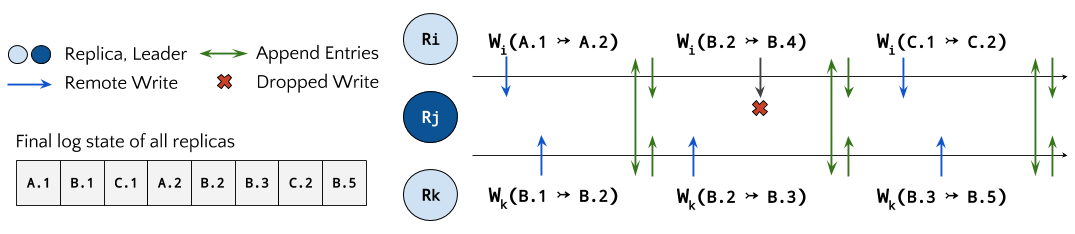
\includegraphics[width=.9\textwidth]{figures/ordered}
        \caption{Sequential ordering in consensus based file system}
        \label{fig:ordered}
\end{figure}

Consider the simple example shown in Figure \ref{fig:ordered}, implemented using the Raft protocol where writes are aggregated in \texttt{AppendEntries} (shown as green lines that occur routinely every heartbeat interval). In this example the object namespace is the set $\{A, B, C\}$ and each version is represented as the object name dot annotated with a monotonically increasing version number (we presume that version 1 of each object has already been written to the log). A write is conducted by reading the latest version of the object and writing the new version, therefore a write by replica $i$ that reads version $n$ and writes to version $m$ on object $O$ is given as follows: $W_i(O.n \rightarrowtail O.m)$.   Writes are ordered with respect to their arrival at the leader ($R_j$), are appended to the logs of the followers on \texttt{AppendEntries}, are committed by the leader when a majority of followers responds affirmative to the append RPC, and are marked as committed by followers on the subsequent \texttt{AppendEntries}. The leader must reject $W_i(B.2 \rightarrowtail B.4)$ in order to maintain consistency because that write would cause a fork to occur in the log. The final log is identically ordered on all replicas for all objects, therefore we can say we have achieved sequential consistency such that every write that appears in log position $i$ happens before ($\rightarrow$) the log entry at $i-1$.

In this example, we have only nominated one \textit{explicit} dependency on each write, the parent version, and enforced a no-forks invariant as a policy on this dependency at the leader. A consequence of this style consistency is the \textit{implicit} causality of all prior writes to a given write. For example, $W_i(C.1 \rightarrowtail C.2)$ implies implicit dependencies on $A.2$ and $B.3$, e.g. any versions that could have possibly been read prior to the write (and also the reason that reads must be logged in order to achieve linearizability). Similarly $W_k(B.3 \rightarrowtail B.5)$ has implicit dependencies on $A.2$ and $C.1$, more closely inspecting the log we can see that $C.2 \rightarrow B.5$ and $C.1 \rightarrow C.2$ therefore by transitivity, $C.1 \rightarrow B.5$, a correct interpretation of the log and implicit dependencies.

While implicit dependencies are critical to consistency, we observe that it is unlikely that a write is truly dependent on every historical write but is rather dependent on a local, recent subset of the namespace \cite{bailis_potential_2012}. Hierarchical consensus therefore makes use of \textit{explicit} causality to allocate the namespace to subquorums in order to balance the leader workload. This has several implications including allowing the ability to lock the ownership of a series of critical files, to specify particular replicas as stable storage for high value data, or to maintain policies and invariants that go beyond ordering; for example spatial polices (what data gets stored), temporal policies (what versions are stored) and synchronization policies (how and when replication occurs).

\subsubsection{Namespace Allocation}

\begin{figure}
    \centering
        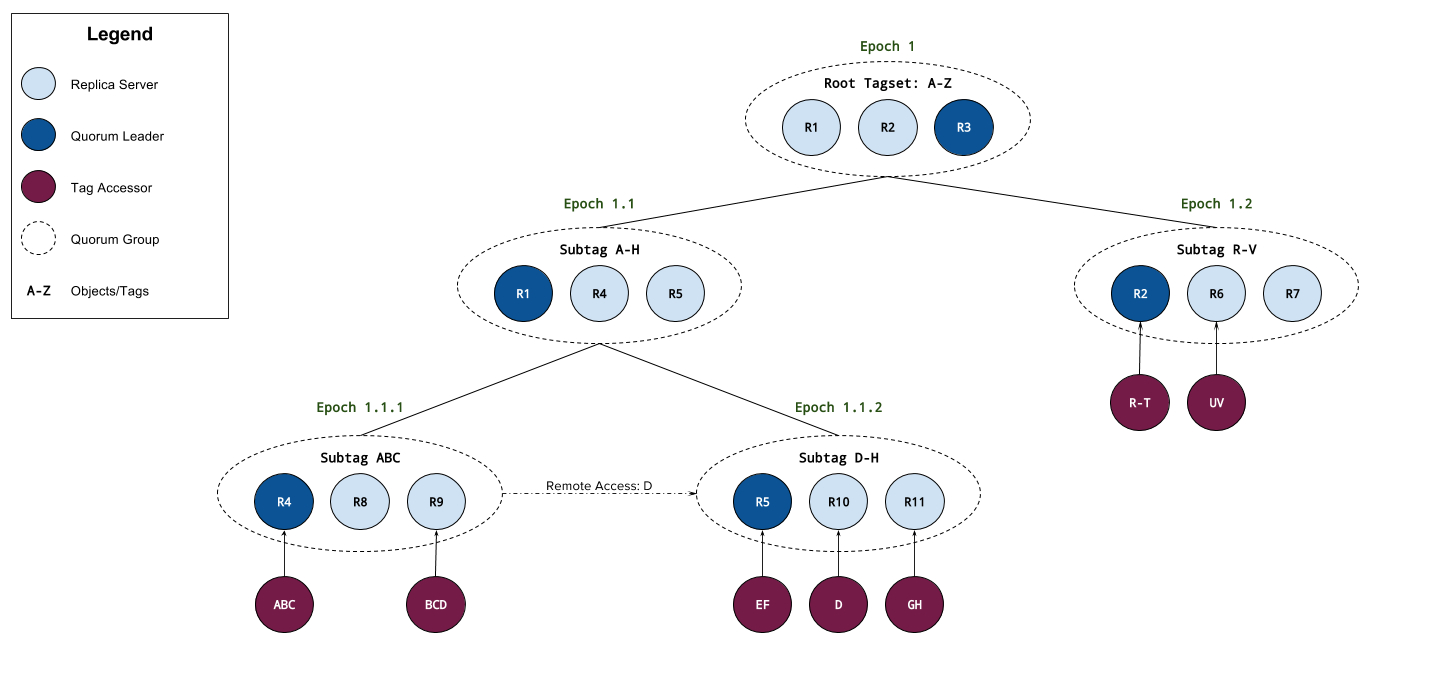
\includegraphics[width=.9\textwidth]{figures/hierarchical}
        \caption{Hierarchical consensus partitions the namespace across subquorums}
        \label{fig:hierarchical}
\end{figure}

An open question for our research is how to automatically allocate the namespace such that leadership of a subset of the namespace is local to the accesses and that members of the quorum are distributed to provide wide area durability and availability. The goal of allocation, is shown in Figure \ref{fig:hierarchical} - a hierarchy of quorums such that the children of each tier manage consensus decisions on a non-overlapping portion of the namespace.

Consider a motivating example using the notion of \textit{sessions}. Starting from a quiescent state (no accesses), a node or a group of nodes begins reading and writing to a set of objects (perhaps collaborative editing of a document, or a series of financial transactions); we expect that after some finite amount of time, the access pattern will change or cease. We can therefore state that all objects involved in a single session are explicitly causally related to each other and to no other objects in the namespace. Whether we describe sessions as a fixed, sliding window or as something more variable, some automatic determination that those objects should be coordinated together is necessary. To that end we will define a \textit{tag} as a time-annotated subset of the namespace and a \textit{tagspace} as the set of non-overlapping tags that compose the namespace for a given time period.

Hierarchical consensus starts with a root quorum whose responsibility is to govern the entire namespace. The root quorum does so by maintaining a root \textit{epoch}, a monotonically increasing counter which identifies the current \textit{tagspace}. In addition to consensus decisions related to leader election, accesses, and membership changes, decisions that modify the tagspace also require consensus. We define two primary operations: \textit{split} creates a new subquorum, splitting a larger tag from the previous tagspace and \textit{join} removes a subquorum, joining two smaller tags from the previous tagspace. Any decision that modifies the tagspace (thus creating a new tagspace) requires an increment of the \textit{epoch}.

The fundamental relationship between accesses in epochs is as follows: any access that happens in epoch $i$ happened before every access in epoch $i-1$; accesses in different tags but in the same epoch happen concurrently from the global perspective, but are ordered locally in the quorum that governs that tag. As a result, every log has a determined, sequentially consistent and correct ordering, though the logs of two individual replicas may differ. Hierarchical consensus cannot provide linearizability, but does provide sequential consistency.

\subsubsection{Operation}

\begin{figure}
    \centering
        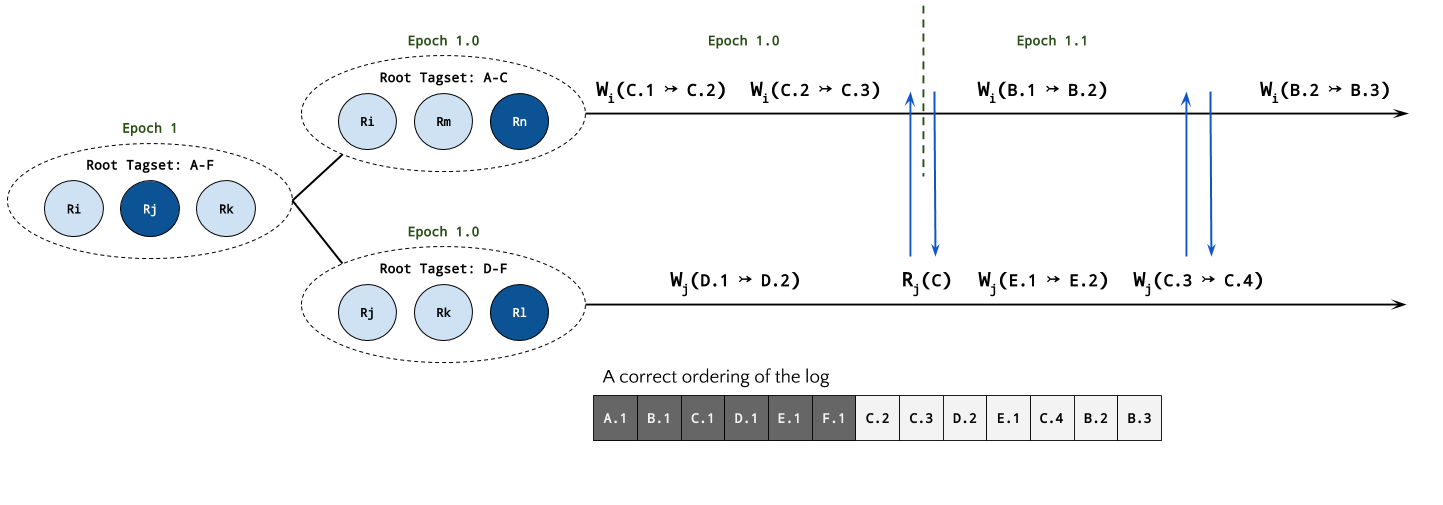
\includegraphics[width=.9\textwidth]{figures/subepoch}
        \caption{Sub-epochs allow remote accesses between tags without a tagspace change.}
        \label{fig:subepoch}
\end{figure}

The namespace allocation creates a tiered structure of leadership such that the root quorum is responsible for the entire namespace, subquorums are responsible for tags, and leaves are responsible for handling accesses to their tag. Any access to an object must be forwarded as a remote access to the leader of the quorum that handles the tag that encapsulates the object. The only exception is the optimization made for members of the quorum who can read locally any object in their tag space. By optimizing the locality of access and spreading the workload to multiple leaders, we hope to show that the overall performance of the system increases.

When a member of a quorum wishes to access an object that is not in that quorum's tag, one of two things must happen: either a tag decision must be made to reallocate the tag space such that it is local to the new accessor or some mechanism must allow remote accesses between quorums. The former case is expensive, but if the accesses to that object become routine then the upfront cost will pay for future accesses. However, for non-routine accesses some mechanism for remote access is required.

The issue is that a remote access from one tag to another creates an implicit dependency between all accesses that happened before the remote access and all those that follow the local one. Correctness is maintained by the ordering of epochs, so some local split is required. Consider the example in Figure \ref{fig:subepoch}: the remote read access, $R_j(C)$ implies any writes to tag $D-F$ following the read depends an all writes in tag $A-C$ that occurred before the read. Furthermore, the remote write $W_j(C.3 \rightarrowtail C.4)$ is a non-conflicting write, depends on all writes on tag $D-F$ that happened before \textit{and} depends on all writes in tag $A-C$ that occurred before the remote read, and occurs concurrently with any writes that happen after so long as there is no conflict.

Our proposed solution is similar to the epoch solution: each tag quorum maintains a per-epoch, monotonically increasing sub-epoch counter. In the case of a remote access, that counter is incremented to demarcate the ordering of all accesses in the tag that happened before the remote access and all those that follow. This counter must be replicated in addition to the version number, and can therefore be seen as an explicit dependency applied to all remote writes. As a result, any quorum that receives these ordering indicators can appropriately order their logs.

This mechanism also leads us to suspect that generalizing the consensus hierarchy to arbitrarily deep levels is possible; particularly since the notion of sub-epoch numbers already exists. Clearly some coordination is required to ensure that tag space changes filter down to all leaf nodes, and that is the primary subject of our future work related to this proposal.

In addition to correctness, we also propose to show failure tolerance by utilize Raft-style quorum mechanics. There are two distinct kinds of failure in a hierarchical system: replica failures (a single node crashes and dies) and partitions, where parts of the network are cut off from receiving messages. We believe that we can model failure tolerance from both of these perspectives through a formulation of quorum size, minimal intersection set between quorums, and the depth/breadth of the hierarchy. We propose to show correctness in the face of failure in the least and will stretch to show inherent robustness due to the structure of the hierarchy.

\subsection{Adaptive Consistency}

Federated Consistency attempts to provide heterogenous devices in a user-centric dynamic cloud the ability to set their consistency level as needed. We propose to show that a small, strong central quorum can improve the global consistency of the system while allowing for local availability. Hierarchical consensus expands the strong central quorum, providing high throughput on the leader of the quorum by allocating multiple leaders for different objects. Together, Federated Consistency and Hierarchical Consensus provide mechanisms that deal with unstable network environments and the unique challenges a multi-user, multi-device system may encounter. However, neither Federated nor Hierarchical deal with the dynamic or mobile nature of the network; and while they provide responsiveness at the user layer, cannot take advantage of boosts in bandwidth or respond to gaps our outages.

Therefore we propose the final step in the study of user-centric dynamic clouds is the real time adaptation of the network according to observed latency values. We have observed that eventually consistent nodes can change their timing parameters at will to take advantage of lower latencies or to save work in sparse network conditions. While joint consensus may be required to adapt the parameters of a consensus group, lowering the timing parameter dramatically improves throughput and commit latency and in the face of increasing latency, ensuring that the timing parameters are conservative enough such that messages aren't received out of order or such that ``leader thrashing'' occurs as much delayed heartbeat messages cause candidacies.

By equipping the system with online monitoring of local network conditions and access patterns, we propose to investigate heuristics and optimizations that can improve performance. In particular, these heuristics can be used to provide a history of performance to the user and recommendations of how to changing timing parameters, topology, or consistency model to adapt. Heuristics can also be used to adapt the policies of different machines in different networks; for example a laptop could participate in hierarchical quorum while at the office or at home, but allow eventual replication while mobile.

Finally, we believe that by constant observing of accesses patterns and the network, we can use machine learning techniques to classify access patterns, detect potential conflicts or anomalies in the network or environment, or to cluster similarly accessed objects to ensure they were always in the same tag. These techniques would automatically and actively adapt the federated system, improving performance in real time and relearning through online techniques and reinforcement from user behavior.

\section{Timeline}

In order to meet the requirements of this proposal and provide substantive results for a dissertation, we propose to undertake the following projects, along with their given priority and timeline.

\begin{center}
\begin{tabular}{|l c|c|}
\hline
Project & Priority & Time Estimate \\
\hline
Simulation of Federated Consistency & $\bigtriangleup$ & 1 months \\
Simulation of Hierarchical Consensus & $\bigtriangleup$ & 2 months \\
Implementation of the FlowFS & $\bigtriangleup$ & 3-4 months \\
Evaluation of FlowFS on real workloads & $\bigtriangleup$ & 2-3 months \\
Proof of correctness and consistency & $\bigtriangleup$ & 1 month \\
Heuristics to optimize and allocate FlowFS & $\bigtriangledown$ & 1 month \\
Online optimization and consistency adaptation & $\bigtriangledown$ & 2-3 months \\
\hline
\multicolumn{2}{|l|}{\textbf{TOTAL}} & 12-16 months \\
\hline
\end{tabular}
\end{center}

After investigations and evaluations of Federated Consistency and Hierarchical Consensus in simulation, I propose to implement a file system utilizing both mechanisms and verify the system meets consistency requirements on large networks in real world workflows. Goals marked with $\bigtriangleup$ indicate necessary checkpoints to the successful completion of the dissertation, including some proof of correctness. I further propose the stretch goals (marked with $\bigtriangledown$) of real time adaptation and online optimization, investigating the application of both heuristics and active machine learning techniques to learn usage patterns and improve consistency and performance.

Based on preliminary work done in simulation as well as the above timeline, I propose the following paper and conference submission goals:

\begin{center}
\begin{tabular}{|l|l|l|c|c|}
\hline
Paper & Title & Location & RFP & Date \\
\hline
Federated Consistency & IEEE ICDCS 2017 & Atlanta, GA & Dec 5, 2016 & Jun 5-8 2017 \\
% http://icdcs2017.gatech.edu/
% IEEE International Conference on Distributed Computing Systems

User-Centric Dynamic Clouds & ACM HotStorage 2017 & Santa Clara, CA & N/A & Jul 10-11, 2017 \\
% https://www.usenix.org/conferences
% ACM Hot Topics in Storage and File Systems 2017

Hierarchical Consensus & ACM PODC 2017 & Washington DC & Feb 10, 2017 & July 2017 \\
% http://www.podc.org/
% ACM Principles of Distributed Computing

Hierarchical FlowFS & ACM SOSP 2017 & Shanghai, China & Apr 21, 2017 & Oct 29-31, 2017 \\
% https://www.sigops.org/sosp/sosp17/index.html
% ACM Symposium on Operating Systems Principles

Responsive Consistency & USENIX NSDI 2018 & N/A & N/A & N/A \\
% https://www.usenix.org/conference/nsdi17
% USENIX Symposium on Networked Systems Design and Implementation

\hline
\end{tabular}
\end{center}

\section{Conclusion}

Distributed storage systems are an important technique to ensuring highly available, durable storage especially in multi-user, collaborative environments. \pjk{Not sure if this sentence is saying anything. At the very least it's weak for the first sentence in the conclusion.}
Replication comes at a cost, however, the need to coordinate replicas to ensure they present a consistent view of the object space. Most of the recent research on coordination and consistency has been in the database context in data centers. However, I propose to study multi-user, heterogenous, mobile systems: user-centric dynamic clouds \pjk{so?}. As the number of computing devices per person increases, and as new devices come online via the Internet of Things; these types of systems in mobile environments will become increasingly important.

We have grounded our proposal in consistency, consensus, and replication. By identifying various consistency levels, we propose that the federation of a variety of consistencies will lead to greater flexibility, and show that consistency is a scale, not discrete categories. Federation will make use of a strong-central quorum to synchronize an eventual cloud, minimizing overall inconsistency in the system. The central quorum needs to be able to scale to dozens or hundreds of does; so to that end we propose Hierarchical Consensus as a means of partitioning consensus decisions to particular objects across the namespace to different leaders. This load balancing will increase throughput but also increase correctness. Finally we propose to explore the automatic adaptation of the network using heuristics or even machine learning. 

\newpage

\appendix
\section{Appendix A: Reading List}
\label{app:readinglist}

\subsection{Consensus}

1) \bibentry{thomas_majority_1979}

2) \bibentry{lamport_paxos_2001}

3) \bibentry{chandra_paxos_2007}

4) \bibentry{lamport_fast_2006}

5) \bibentry{ongaro_search_2014}


\subsection{Consistency}

1) \bibentry{lamport_time_1978}

2) \bibentry{terry_managing_1995}

3) \bibentry{bailis_quantifying_2014}

4) \bibentry{bailis_potential_2012}

5) \bibentry{bermbach_consistency_2013}


\subsection{Replication}

1) \bibentry{stoica_chord:_2001}

2) \bibentry{kubiatowicz_oceanstore:_2000}

3) \bibentry{gray_dangers_1996}

4) \bibentry{venkataramani_operating_2002}

5) \bibentry{almeida_version_2002}



% \newpage

% \section{Appendix B}
% \label{app:cvtdp2r}


\newpage

\bibliographystyle{plain}
\bibliography{prelim}

\end{document}
